\documentclass[a4paper,11pt]{article}

% Packages for additional functionality
\usepackage[utf8]{inputenc} % For UTF-8 encoding
\usepackage{amsmath, amssymb} % For math symbols
\usepackage{hyperref} % For hyperlinks
\usepackage{listings} % For code blocks
\usepackage{xcolor} % For syntax highlighting in code
\usepackage{graphicx}
% Customize hyperlink colors
\hypersetup{
    colorlinks=true,
    linkcolor=blue,
    filecolor=magenta,
    urlcolor=cyan,
}

% Set the default font style
\renewcommand{\familydefault}{\sfdefault}

\newcommand{\uninuvola}{UniNuvola }
\newcommand{\uninuvolan}{UniNuvola}
\newcommand{\jupyterhub}{Jupyterhub }
\newcommand{\jupyterhubn}{Jupyterhub}

\newcommand{\doctitle}{Complete UniNuvola Guide}
\newcommand{\docsubtitle}{TODO}

% Code block style
\lstset{
    basicstyle=\ttfamily\small,
    backgroundcolor=\color{lightgray},
    frame=single,
    breaklines=true,
    postbreak=\mbox{\textcolor{red}{$\hookrightarrow$}\space},
}

% Document starts
\begin{document}

% frontmatter.tex
\begin{titlepage}
    \thispagestyle{empty}
    \begin{center}
        % Logo
        \vspace*{1.5cm}
        
\includegraphics[width=0.7\textwidth]{img/uninuvola_logo.jpeg} % <-- Replace with your logo

        % Organization Name
        %\vspace{1cm}
        %{\Large \textsc{My Organization Name}} % <-- Replace with your org name

        % Document Title
        \vspace{2.5cm}
        {\Huge \bfseries \doctitle} \\[1ex] % <-- Replace with your title

        % Subtitle (optional)
        {\large \textit{\docsubtitle}} % <-- Replace or remove

        % Author(s)
        \vspace{2.5cm}
        {\large \textbf{The UniNuvola Team}} \\[0.5ex] % <-- Replace with actual names

        % GitHub Issue
        \vspace{2.5cm}
        {\large For any issue please report it using the GitHub page: \href{https://github.com/UniNuvola/UniNuvola}{UniNuvola}}
        % Update Date
        \vfill
        {\normalsize Last Updated: \today} % <-- Or replace \today with a fixed date

        % Footer (optional)
        % TODO: delate or keep ??
        \vspace{1cm}
        {\small © \the\year\ University of Perugia. All rights reserved.} % <-- Update as needed
    \end{center}
\end{titlepage}

\part{Quickstart Guide}
\section{Introduction}

Welcome to this quickstart guide for using UniNuvola. This is not a comprehensive manual—one will be made available
soon—but it provides the information required to start using the prototype server.

\section{Accessing the server}

You can access UniNuvola via web browser, using the University VPN, through the
\href{https://www.uninuvola.unipg.it/}{https://www.uninuvola.unipg.it/} website. You will be redirected to the UniNuvola
Vault login page. After selecting the LDAP option (Figure \ref{fig:login}) in the drop-down menu, you can enter your
login details: these are the same as those you use to access the University services (user id and password). If it is
your first time accessing the server, you will be redirected to a web page  where you will automatically request access
to the infrastructure. Access will be granted once one of the operators approves your request (Figure
\ref{fig:pending}). If you already have an account, or after you get accepted you will redirected to the image and
resources selection page.


\begin{figure}[!ht]
    \centering
    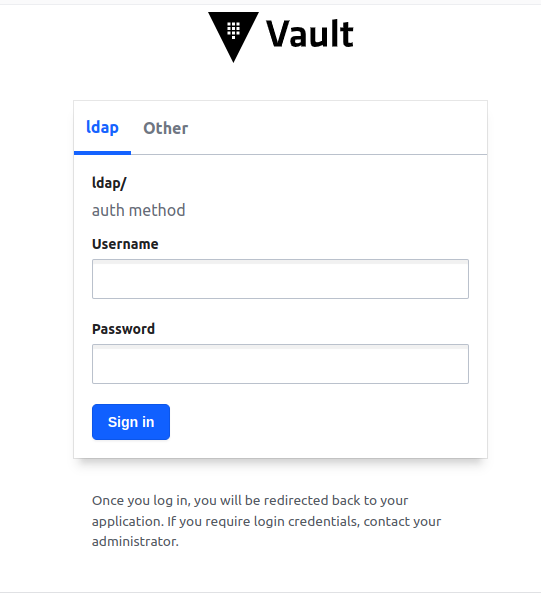
\includegraphics[width=0.5\linewidth]{img/login_page.png}
    \caption{UniNuvola's login page.}
    \label{fig:login}
\end{figure}



\begin{figure}[!ht]
    \centering
    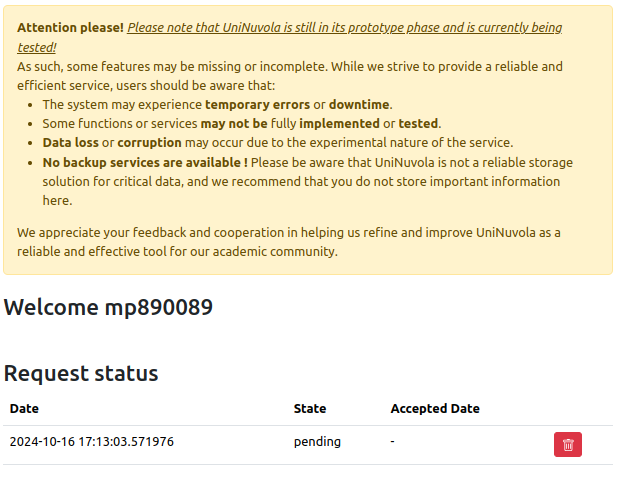
\includegraphics[width=0.5\linewidth]{img/request_page.png}
    \caption{Pending acceptance page}
    \label{fig:pending}
\end{figure}

\section{Selection of the Image and resources}

\textbf{Note:} This section will undergo further modifications within the next month, and the quickstart will be updated
accordingly. \\

After a successful login, you will be directed to the resource selection page. The first section to complete is the
image selection. This part needs to be filled in by the user or select one of the available options. Images can be
selected from those available in UniNuvola (see table \ref{tab:images}) or from your own customised version on
Dockerhub. The tags \textit{latest} and \textit{deployed} are available in our harbor repository.\\

\begin{table}[]
    \caption{List of the official images in UniNuvola}
    \label{tab:images}
    \centering
    \begin{tabular}{|c|c|}
        \hline
        Base              & harbor1.fisgeo.unipg.it/uninuvola/base             \\ \hline
        Engineering       & harbor1.fisgeo.unipg.it/uninuvola/engineering      \\ \hline
        Conda             & harbor1.fisgeo.unipg.it/uninuvola/conda            \\ \hline
        Chemistry         & harbor1.fisgeo.unipg.it/uninuvola/chemistry        \\ \hline
        Quantum Computing & harbor1.fisgeo.unipg.it/uninuvola/quantumcomputing \\ \hline
        Genomics          & harbor1.fisgeo.unipg.it/uninuvola/genomics         \\ \hline
        Hydraulics        & harbor1.fisgeo.unipg.it/uninuvola/hydraulics       \\ \hline
        Tensorflow        & harbor1.fisgeo.unipg.it/uninuvola/tensorflow       \\ \hline
        Pytorch           & harbor1.fisgeo.unipg.it/uninuvola/pytorch          \\ \hline
        Pytorch-GPU       & harbor1.fisgeo.unipg.it/uninuvola/pytorchgpu       \\ \hline
        Optimisation      & harbor1.fisgeo.unipg.it/uninuvola/optimisation     \\ \hline
    \end{tabular}
\end{table}


The image name will appear as:
\begin{lstlisting}[language=bash] 
harbor1.fisgeo.unipg.it/uninuvola/base:deployed
\end{lstlisting}

In the next drop-down menus, you will choose the number of CPUs required (1, 2, 4, 8, 16, 32), the amount of RAM
required (4 Gb, 8 Gb, 16 Gb, 32 Gb), and, if you require GPUs, the number of them (0, 1, 2, 3, 4). At the moment, 100
gigabyte of persistent storage are available for each user (Figure \ref{fig:resources}).\\

\begin{figure}[!ht]
    \centering
    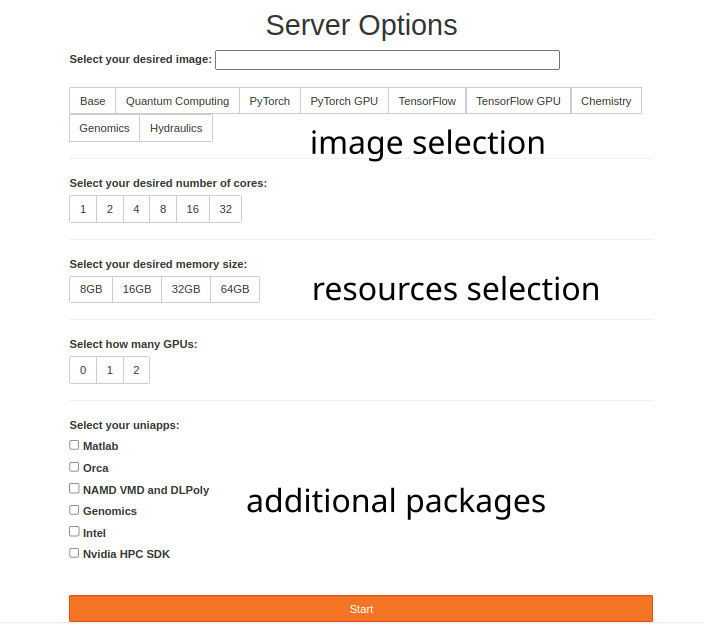
\includegraphics[width=0.75\linewidth]{img/resource_selection.png}
    \caption{Resources selection page}
    \label{fig:resources}
\end{figure}

As per the disclaimer in Figure \ref{fig:pending}, remember: \textbf{UniNuvola is a prototype. We provide computational
    power and storage, but data are not backed up. Be careful with your data!} \\

\section{Inside UniNuvola}
The main page of UniNuvola appears as depicted in Figure \ref{fig:uninuvola_main_page}. The top bar allows some
management actions and some customisation of the user interface. Most importantly, inside the file men, you can find the
disconnect and  the control hub options. The former allows to connect and disconnect from Jupyter (be aware that you
will disconnect from the Hub page, but the pod will continue run up to 12 hours after becoming inactive), the later
option allows to kill the running image and it allows the user to load a new image. \\

the left side of the menu allows the management of the local files. The four most upper options allow the user in order
to: open new launchers tabs, create new directories, upload files, and refresh the browser. Files can be moved through
the web interface or through remote terminal connection from UniNuvola to the machine hosting the files.\\

The orange square includes all Python and R toolkits. The top part includes all the environments notebooks in the image,
the bottom part instead the relative consoles. The top right part, the purple square, contains the Xpra notebook, that
allows the usage of programs requiring a graphical interface.  \\

In the last line, the first element, circled in green, allows the user to use a terminal. All terminals will start with
the sh/bash terminal depending on the image. The elements circled in blue are the text editors in the Hub,  in the case
of the figure a general text editor, a Markdown and a Python file editor. \\


\begin{figure}[!ht]
    \centering
    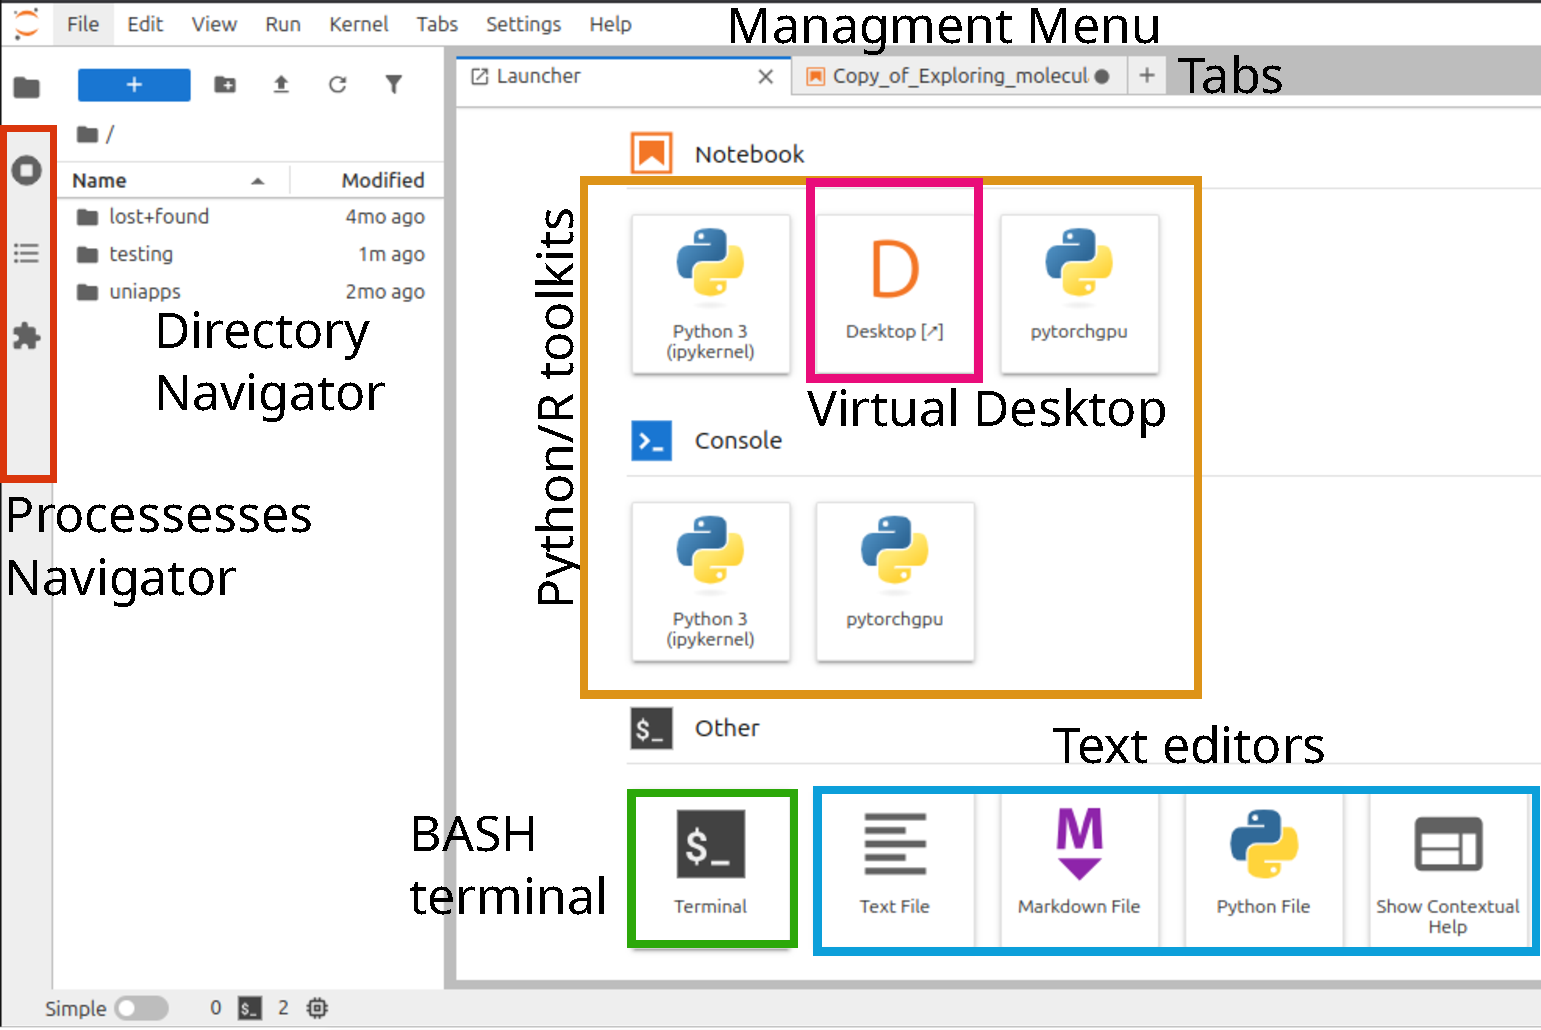
\includegraphics[width=0.8\linewidth]{img/uninuvola.pdf}
    \caption{Example of Jupyter Lab interface in UniNuvola.}
    \label{fig:uninuvola_main_page}
\end{figure}

Each user has the possibility of create 5 Jupyter  named nodes that can be used as scratch space. The option can be
found in the Hub Control Panel into the File menu. Figure \ref{fig:uninuvola_multi} shows an example page.

\begin{figure}[!ht]
    \centering
    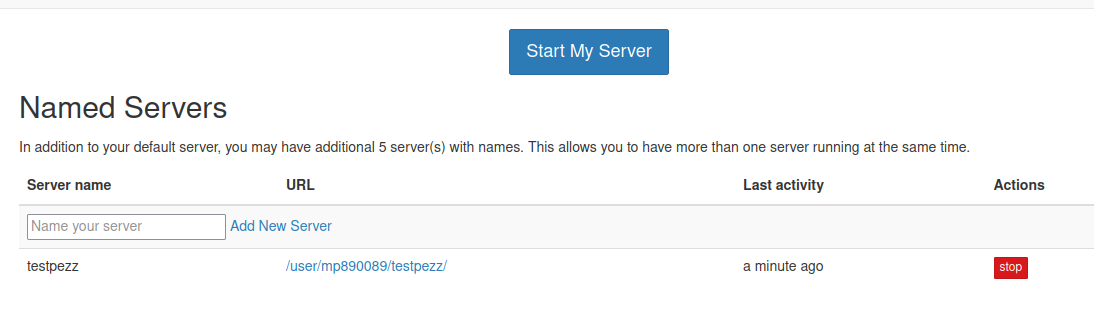
\includegraphics[width=0.90\linewidth]{img/multiserver.png}
    \caption{Named server page example}
    \label{fig:uninuvola_multi}
\end{figure}

\section{Activation of the conda environment}
The first time an user enters in UniNuvola or deletes the .bashrc, conda is not active in the terminal. At this stage
the process can be done manually following these steps:
\begin{lstlisting}[language=bash] 
/opt/conda/condabin/conda  init source ~/.bashrc
\end{lstlisting}
Afterwards, you will be able to use conda as in any other environment.

\section{Troubleshooting}
\subsection{Multiple readdressing into the login page}
If you didn't logout after your account creation, or your token expired, it is possible that in the following session
you can be readdressed into the login page.  In order to solve the issue you can opt for two solutions:
\begin{itemize}
    \item[\textbf{I}] disconnect by hand from the UniNuvola Vault page.
    \item[\textbf{II}] delete the cookies in your browser.
\end{itemize}

To achieve the fist step, you will need to connect to the
\href{https://vault.uninuvola.unipg.it:8200/ui/vault/dashboard}{UniNuvola Vault webpage}, press on the icon representing
a person and than click logout. Figure \ref{img:logout} shows the process.      \\
\begin{figure}[!h]
    \center
    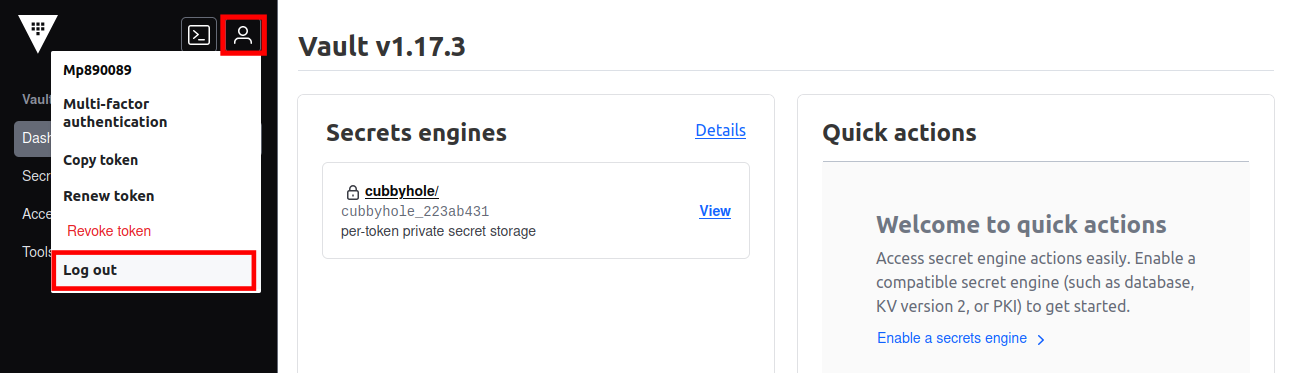
\includegraphics[width=0.8\linewidth]{img/vault.png}
    \caption{Uninvola's Vault logout page.}
    \label{img:logout}
\end{figure}

Afterwards you should be able to reaccess to UniNuvola.

\newpage

\part{Custom Image}
\section{Anatomy of the UniNuvola Images system}\label{image_anatomy}
\uninuvola's images are a collection of container images recipes that are
available in the UniNuvola's GitHub \href{https://github.com/UniNuvola/images}
{images repository}. 
These images have been created by the UniNuvola team and are available for all users.
The base of all images is the jupyter notebook image, a system widely used in the
scientific community, extended with many packages to cover a wide range of
scientific applications commonly used in our University.

The images can be seen as a tree structure, where the root is the base image
``base'' and the branches adds new features to the base image and eventually 
are the origin of different leaves. 
For example, the image ``base/conda`` brings the conda package manager to the base
image, while ``base/conda/pytorch`` adds the pytorch package to the conda image.

With this in mind, building a new image is as simple as copying one of the
available recipes, modifying it to your needs and building a new image.
To ease this process, we have created a public template for the images creation.

\section{Re-creation of the base image}\label{image_recreation}
Let's see how to create a replica of the base image with a different name and belonging to the user.

\begin{bclogo}[logo=\bcinfo, couleurBarre=orange, noborder=true, couleur=white]{Warning}
  Pre-requisite: you need to have a github account to replicate the base
  image. You can use your personal account or create a new one.
\end{bclogo}

Login to your github account and go to the UniNuvola's \href{https://github.com/UniNuvola/custom-image-template}{custom image template}
repository. Click on the ``Use this template'' button to create a new
repository based on the template. This will create a new repository in your
github account with the same structure as the template. You can name it
any name you like. \\
This simple action trigger a github action that will automatically build
the image and push it to the GitHub registry. The action will take a few
minutes to complete. You can check the progress of the action by going to the ``Actions'' tab of
your new repository. \\
Once the action is completed, you will see a new image in your GitHub
repository. You can check the image by going to the ``Packages'' tab of your
repository.
\\
By clicking on the image name, you will see the details of the image, including
the full name of the image, that should be in the format: \\
\\
``ghcr.io/\textit{your\_github\_username}/\textit{your\_repository\_name}:main''
\\
\\
You can use this name to run the image in your UniNuvola environment, by
putting it in the ``Select your desired image'' field of the
\jupyterhubn{} interface. \\
\section{Customizing the image}\label{image_customization}
The main part of the image creation is done by modifying the Dockerfile. The
Dockerfile is a text file that contains all the instructions to build the
Docker image. The Dockerfile is located in the root directory of your
repository and contains a placeholder for the custom code:
\begin{lstlisting}[language=python]
  ## -- ADD YOUR CODE HERE !! -- ##

  ## --------------------------- ##
\end{lstlisting}
This is the place where you can add your custom code. You can add any
Dockerfile command you like. Take a look at the \href{https://github.com/UniNuvola/images}
{UniNuvola images repository} to see some examples of Dockerfiles we have
created. \\
You can either modify the file directly in the github interface or clone the
repository to your local machine and modify it there. If you choose the
latter option, you will need to push the changes to your github repository
after you are done. \\
In any case, every time you push a change to the repository, the github action will
automatically build the image and push it to the GitHub registry, as described in
the previous section. \\
Cloning the repository to your local machine is a good option since you 
can use your favorite text editor to modify the Dockerfile. You can also
build the image locally and check if it builds correctly before pushing it to
github. To do this, you will need to have a container engine installed on
your local machine, like Docker. \\
Describing how to install and use locally a container runtime is out of the scope of this document.

\subsection{Some examples of Dockerfile commands}

TODO Finish

You can install new packages using the appropriate package managers, using the
\textit{RUN} keyword in the Dockerfile

\begin{lstlisting}[language=python]
  RUN apt-get update && apt-get install -y package\_name
\end{lstlisting}

Copy your application code into the Docker image, using the \textit{COPY} (for
local files) or \textit{ADD} (for local and remote files) command in the
Dockerfile. Do not use the /home directory as the target directory as it will be
overwritten when loading the external storage.

\begin{lstlisting}[language=python]
  COPY myfile.txt  /app
  ADD https://example.com/path/to/remote/file.txt /app/
\end{lstlisting}


\end{document}
